\documentclass{jsarticle}
\usepackage[dvipdfmx]{graphicx}
\usepackage{float}
\usepackage{amsmath}
\usepackage[dvipdfmx]{color}
\usepackage{listings}
\usepackage{subfigure}
\begin{document}
\title{小野寺研インターン}
\author{澤 孝晃}
\maketitle

\section{序論}

今回のインターンでは、微細デバイスに発生するランダムテレグラフノイズ(RTN)をリング発振回路を用いて測定し、RTNが回路性能の最悪分布に与える影響を評価する。測定対象であるRTNは統計的な性質を持っており、各種統計的な性質をモデル化することが目的である。統計的な評価を行うために、同じ寸法の大量のデバイスの電流特性の時間変化を測定し、デバイス毎に観測される電流値変動の振幅および捕獲・放出するまでの平均時間などを測定する。

\section{方法}

今回の測定環境では、FPGAボードとPCを使って、スロット0からスロット71のリングオシレータ(RO)を、セクション0からセクション383まで384個のセクションの発信周波数を測定する。各セクションそれぞれ10秒ずつ1msの間隔で測定するため、1つのリングオシレータに対して1時間程度かかる。

\section{正規化前の結果}

\begin{figure}[H]
	\centering
	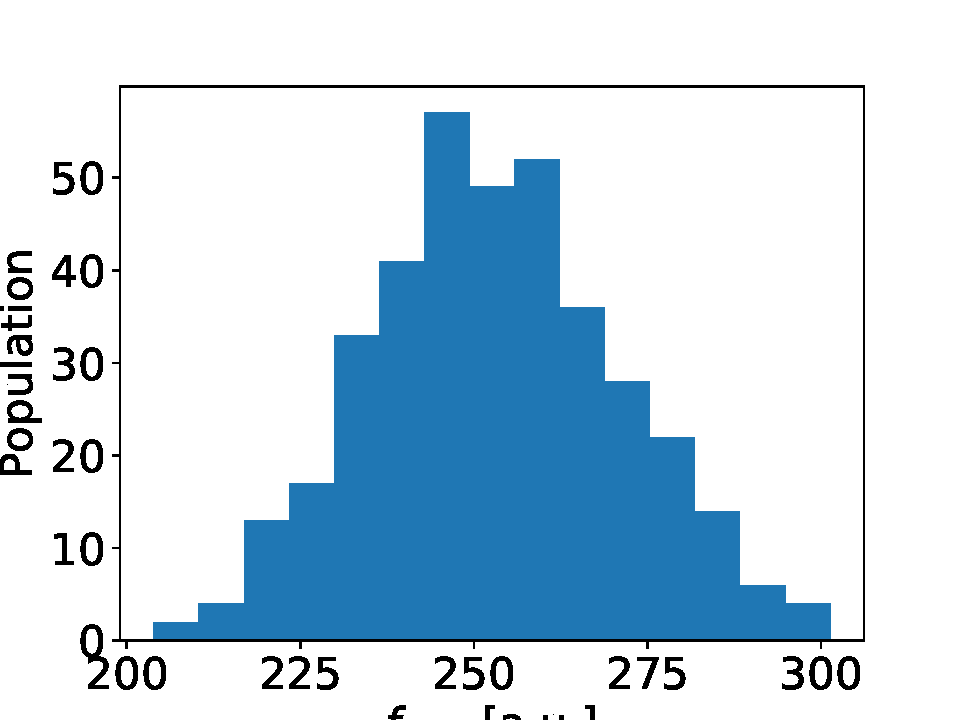
\includegraphics[width=8cm]{../fig_max_hist/180518_ch02v050r0d3_int252_time10000_fig_max_hist.pdf}
	\label{fig:fig_max_hist/180518_ch02v050r0d3_int252_time10000_fig_max_hist.pdf}
\end{figure}

\begin{figure}[H]
	\centering
	\subfigure[7段]{
		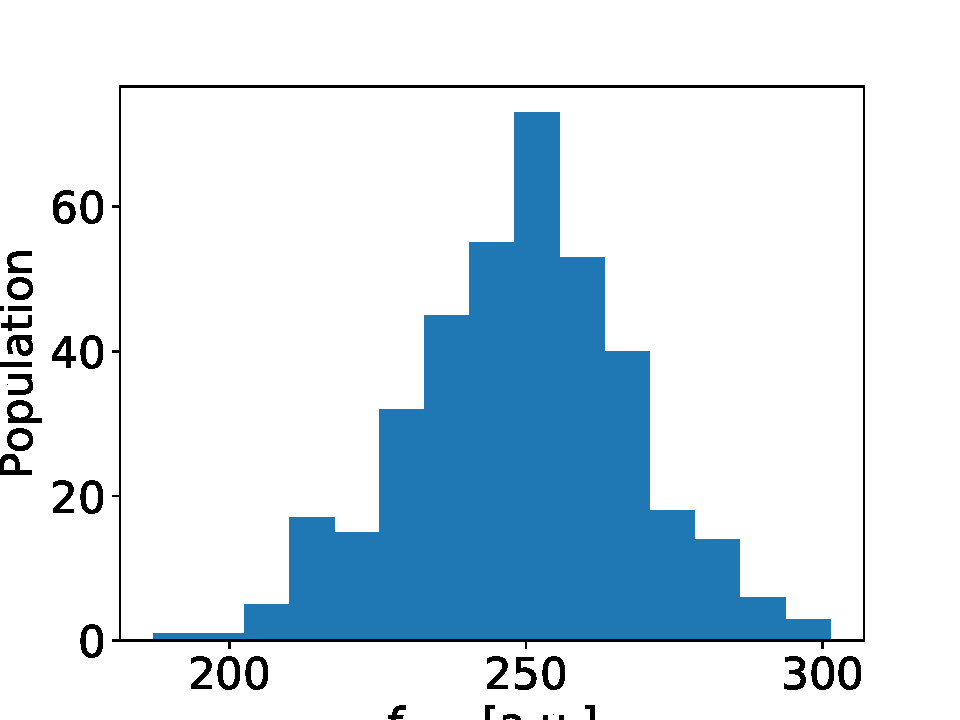
\includegraphics[width=4cm]{../fig_max_hist/180522_ch02v050r36d3_int247_time10000_fig_max_hist.pdf}
		\label{fig:fig_delta_qqplot/180522_ch02v050r36d3_int247_time10000_fig_delta_qqplot.pdf}
	}
	\subfigure[13段]{
		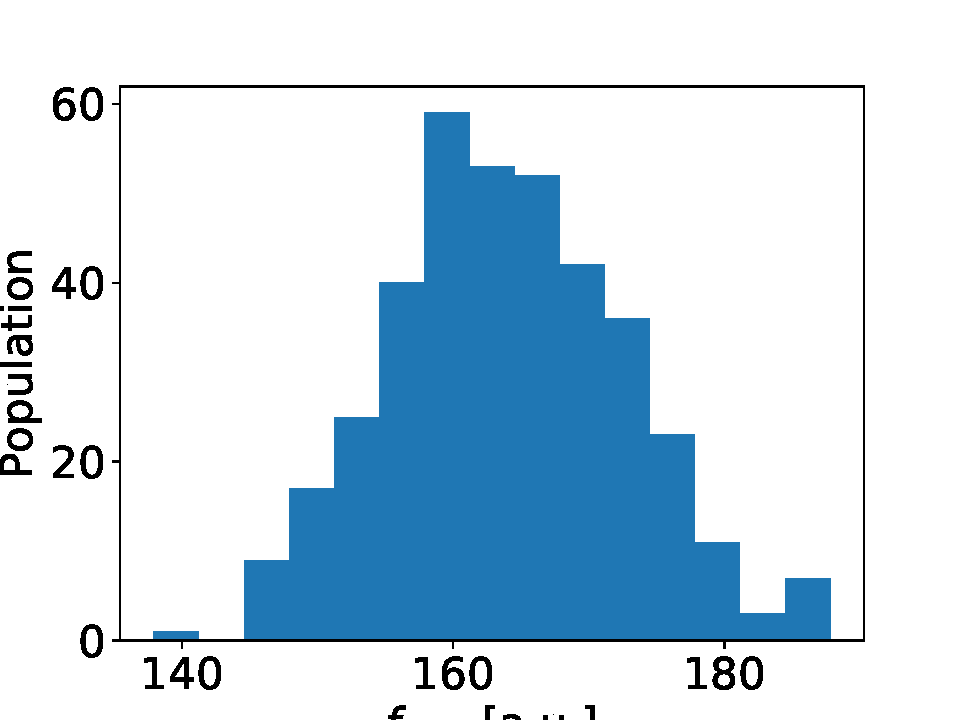
\includegraphics[width=4cm]{../fig_max_hist/180522_ch02v050r41d3_int163_time10000_fig_max_hist.pdf}
		\label{fig:fig_delta_qqplot/180522_ch02v050r41d3_int163_time10000_fig_delta_qqplot.pdf}
	}
	\subfigure[19段]{
		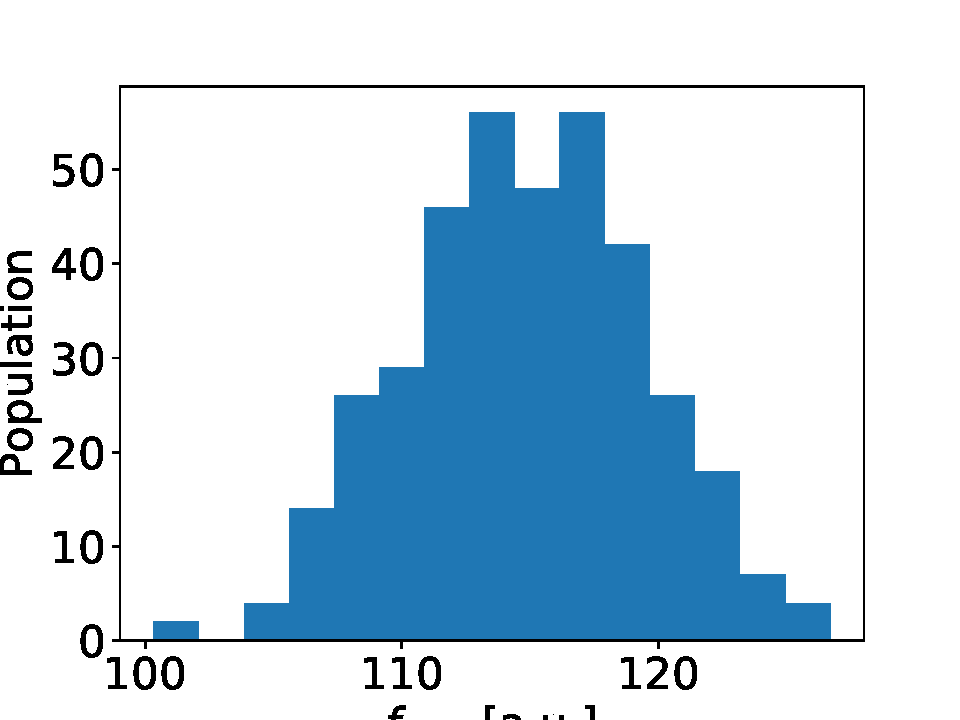
\includegraphics[width=4cm]{../fig_max_hist/180522_ch02v050r42d3_int114_time10000_fig_max_hist.pdf}
		\label{fig:fig_delta_qqplot/180522_ch02v050r42d3_int114_time10000_fig_delta_qqplot.pdf}
	}
	\subfigure[29段]{
		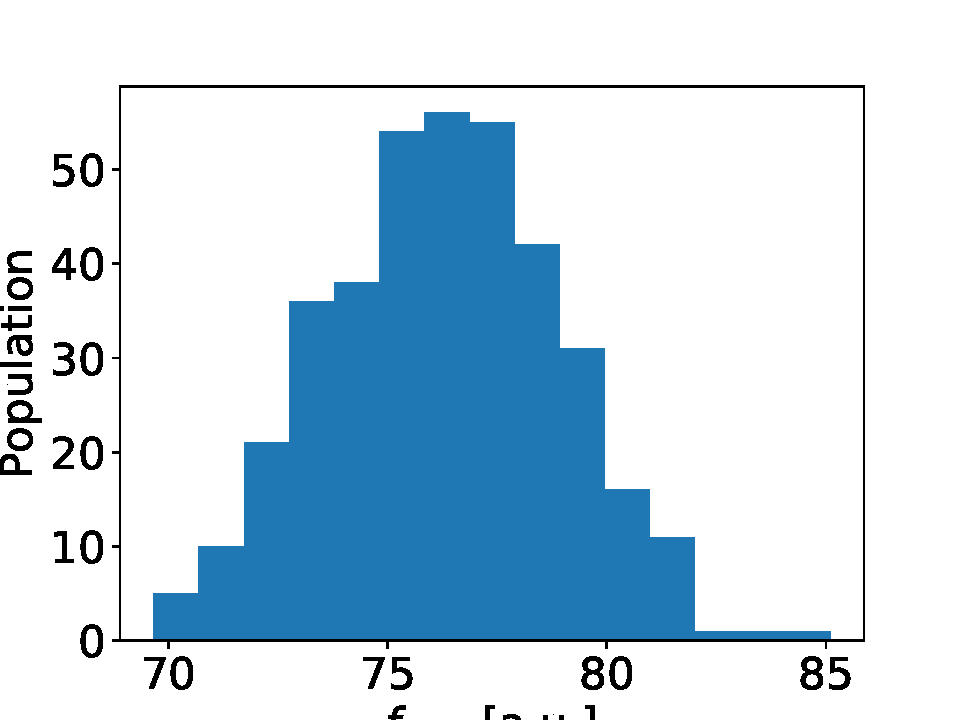
\includegraphics[width=4cm]{../fig_max_hist/180522_ch02v050r43d3_int75_time10000_fig_max_hist.pdf}
		\label{fig:fig_delta_qqplot/180522_ch02v050r43d3_int75_time10000_fig_delta_qqplot.pdf}
	}
	\subfigure[59段]{
		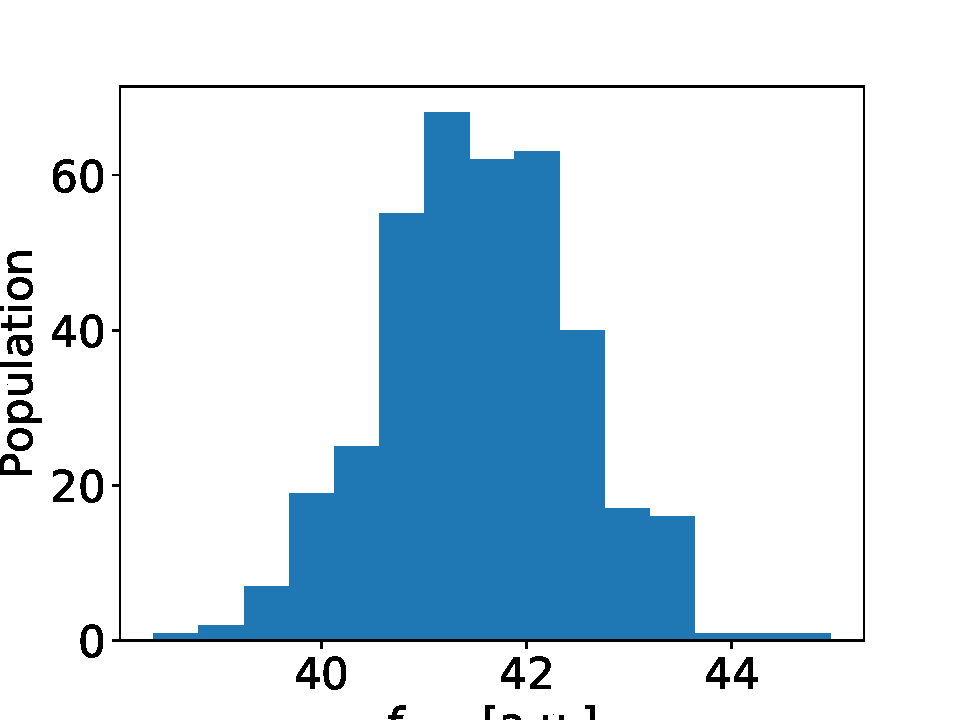
\includegraphics[width=4cm]{../fig_max_hist/180522_ch02v050r44d3_int41_time10000_fig_max_hist.pdf}
		\label{fig:number_of_network_operations_comparison_5}
	}
	\caption{Number of network operations comparison}
	\label{fig:number_of_network_operations_comparison}
\end{figure}



\begin{figure}[H]
	\centering
	\includegraphics[width=8cm]{../fig_max_qqplot/180518_ch02v050r0d3_int252_time10000_fig_max_qqplot.pdf}
	\label{fig:fig_max_qqplot/180518_ch02v050r0d3_int252_time10000_fig_max_qqplot.pdf}
\end{figure}

\section{正規化後の結果}

\begin{figure}[H]
	\centering
	\includegraphics[width=8cm]{../fig_delta_hist/180518_ch02v050r0d3_int252_time10000_fig_delta_hist.pdf}
	\label{fig:fig_delta_hist/180518_ch02v050r0d3_int252_time10000_fig_delta_hist.pdf}
\end{figure}

\begin{figure}[H]
	\centering
	\subfigure[7段]{
		\includegraphics[width=5cm]{../fig_delta_hist/180522_ch02v050r36d3_int247_time10000_fig_delta_hist.pdf}
		\label{fig:fig_delta_qqplot/180522_ch02v050r36d3_int247_time10000_fig_delta_qqplot.pdf}
	}
	\subfigure[13段]{
		\includegraphics[width=5cm]{../fig_delta_hist/180522_ch02v050r41d3_int163_time10000_fig_delta_hist.pdf}
		\label{fig:fig_delta_qqplot/180522_ch02v050r41d3_int163_time10000_fig_delta_qqplot.pdf}
	}
	\subfigure[19段]{
		\includegraphics[width=5cm]{../fig_delta_hist/180522_ch02v050r42d3_int114_time10000_fig_delta_hist.pdf}
		\label{fig:fig_delta_qqplot/180522_ch02v050r42d3_int114_time10000_fig_delta_qqplot.pdf}
	}
	\subfigure[29段]{
		\includegraphics[width=5cm]{../fig_delta_hist/180522_ch02v050r43d3_int75_time10000_fig_delta_hist.pdf}
		\label{fig:fig_delta_qqplot/180522_ch02v050r43d3_int75_time10000_fig_delta_qqplot.pdf}
	}
	\subfigure[59段]{
		\includegraphics[width=5cm]{../fig_delta_hist/180522_ch02v050r44d3_int41_time10000_fig_delta_hist.pdf}
		\label{fig:number_of_network_operations_comparison_5}
	}
	\caption{Number of network operations comparison}
	\label{fig:number_of_network_operations_comparison}
\end{figure}

\begin{figure}[H]
	\centering
	\subfigure[7段]{
		\includegraphics[width=5cm]{../fig_delta_qqplot/180522_ch02v050r36d3_int247_time10000_fig_delta_qqplot.pdf}
		\label{fig:fig_delta_qqplot/180522_ch02v050r36d3_int247_time10000_fig_delta_qqplot.pdf}
	}
	\subfigure[13段]{
		\includegraphics[width=5cm]{../fig_delta_qqplot/180522_ch02v050r41d3_int163_time10000_fig_delta_qqplot.pdf}
		\label{fig:fig_delta_qqplot/180522_ch02v050r41d3_int163_time10000_fig_delta_qqplot.pdf}
	}
	\subfigure[19段]{
		\includegraphics[width=5cm]{../fig_delta_qqplot/180522_ch02v050r42d3_int114_time10000_fig_delta_qqplot.pdf}
		\label{fig:fig_delta_qqplot/180522_ch02v050r42d3_int114_time10000_fig_delta_qqplot.pdf}
	}
	\subfigure[29段]{
		\includegraphics[width=5cm]{../fig_delta_qqplot/180522_ch02v050r43d3_int75_time10000_fig_delta_qqplot.pdf}
		\label{fig:fig_delta_qqplot/180522_ch02v050r43d3_int75_time10000_fig_delta_qqplot.pdf}
	}
	\subfigure[59段]{
		\includegraphics[width=5cm]{../fig_delta_qqplot/180522_ch02v050r44d3_int41_time10000_fig_delta_qqplot.pdf}
		\label{fig:number_of_network_operations_comparison_5}
	}
	\caption{Number of network operations comparison}
	\label{fig:number_of_network_operations_comparison}
\end{figure}



\end{document}
